Predstavljanje argumenata u računalima moguće kroz standardne 
serijalizacijske formate, kao što su
XML \engl{Extensible Markup Language} ili JSON \engl{JavaScript Object Notation}. 
No, radi se generičkim formatima, koji ne poznaju specifičnosti 
strukture argumenata. Nezavisno razvijeni alati 
za analizu argumentacije kao Araucaria \citep{reed2004araucaria},
Rationale \citep{van2007rationale}
ili Carnedeas \citep{gordon2006carneades}
su razvili vlastiti serijalizacijski format pohrane
argumenata. Kako je potreba za integracijom između tih alata rasla, tako
je i rasla potreba za ujedinjenim formatom za pohranjivanje argumenta. 

\section{AIF}

Standardizacija definiranja računalnog jezika bila je nužna zbog tri glavna razloga:
\begin{enumerate}
    \item razmjena dokumenata kroz različite programske agente (primjerice 
korištenje dokumenata kreiranih u Araucarii u Rationaleu i obratno), 
    \item kompatiblinost argumentacijskih teorija u različitim programskim agentima
(primjerice, Araucaria koristi Toulminovu teoriju, dok Rationale samo poznaje 
Waltonove argumentacijske teorije \citep{walton2012argument}, te 
    \item potrebe da se automatski procesiraju logičke izjave
\end{enumerate}

Prije AIF-a bilo je nekoliko pokušaja stvaranja zajedničkog jezika, ponajprije
Araucarin AML \engl{Argument Markup Language}. AML, baziran na XML-u
\engl{Extensible Markup Language} osmišljen je za označavanje i analizu
argumentacije u prirodnom jeziku. Sintaksa AML jezika specificirana je pomoću
DTD \engl{Document Type Definition} strukturalnih ograničenja.  
2005.\ nastao je prvi prijedlog za \textbf{AIF} \engl{Argument
Interchange Format} jezik \citep{chesnevar2006towards}. 
Baziran na dobro poznatom RDF jeziku, ideja AIF-a
je bila ponuditi dovoljnu ekspresivnost kojom bi se obuhvatile sve
općeprihvaćene teorije argumentacije i efikasno pohranili 
argumenti u računalima. 
AIF je 2008.\ dobio proširenje za dijalog \citep{reed2008aif+}.
Začetak AIF-a se smatra prvim korakom
prema ostvarivanju argument web-a. 


\section{Specifikacija AIF-a}

AIF odlikuju 
\begin{enumerate*}
    \item sintaksa razumljiva programskim agentima,
    \item eksplicitna semantika,
    \item koncepti i proširenja te
    \item objedinjen apstraktni model koncepata i relacija između
koncepata.
\end{enumerate*}

\subsection{Koncepti i relacije}

Objekti argumentacije predstavljaju se kao skup čvorova povezanih usmjerenim grafom. 
Neformalno se takav usmjereni graf u kontekstu argumentacije naziva
argumentativnom mrežom \engl{argument network} \textbf{AN}. Ne 
postoje nikakva ograničenja na oblik grafa koji može poprimiti AN.

\subsection{Čvorovi}

Razlikujemo dvije osnovne vrste \textbf{čvorova}: informacijske čvorove
\engl{information nodes} I-čvorove i shematske \engl{scheme nodes} S-čvorove.
I-čvorovi predstavljaju sadržaj izjava i čvrsto su povezani s temom
argumentativne rasprave, S-čvorovi predstavljaju primjenu obrazaca u
argumentiranju i smatraju se neovisnim o argumentativnoj raspravi. Postoje tri
osnovna tipa obrasca u argumentiranju: posljedica \engl{inference},
preferiranje \engl{preference} i sukob \engl{conflict}. Primjena sheme
radi se kroz S-čvor koji sukladno vrstama obrazaca u argumentiranju može biti
čvor primjene logičke posljedice \engl{inference application node} (\textbf{RA-čvor}), 
čvor primjene preferiranja \engl{preference application node} (\textbf{PA-čvor}) te
čvor primjene sukoba \engl{conflict application node} (\textbf{CA-čvor}).

\subsection{Bridovi}

\textbf{Čvorovi} su povezani usmjerenim bridovima. Kažemo da brid povezuje čvorove $A$ i $B$
tako da ide iz početnog čvora $A$ u odredišni čvor $B$. Razlikujemo shematske i podatkovne
bridove. Početne točke shematskih bridova su S-čvorovi, dok su početne točke 
podatkovnih bridova I-čvorovi. Primjerice, čvorovi $A$ i $B$ su povezani usmjerenim bridom 
$A \rightarrow B$. Ukoliko je čvor $A$ početna točka tipa
S-čvor primjene logičke posljedice RA-čvor onda je čvor $B$ zaključak strukture
čvora $A$. Čvor $B$ može biti S-čvor ili I-čvor. Ukoliko je početni čvor I-čvor onda
odredišni čvor može biti samo S-čvor. 
Ideja iza toga stoji u principu da nije moguće povezati dvije izjave bez da se
specifira relacija (S-čvor) između izjava. 
\cite{chesnevar2006towards} navode sve moguće kombinacije S-čvorova i I-čvorova
sa bridovima uz pripadajuće semantičko značenje. 

\section{Primjer AIF dokumenta}

Primjer isječka AIF dokumenta u RDF formatu vidljiv je kodu~\ref{lst:aif_rdf}.
Tip čvora definiran je kroz \textit{rdf:type} (I-čvor ili S-čvor),
\textit{aif:claimText} predstavlja sadržaj I-čvora, dok S-čvor ima različita
svojstva (ovisno o tome radi li se o RA, PA ili CA čvoru). 
U ovom primjeru imamo S-čvor zaključivanja (RA-čvor) koji nam govori
koji spaja dva čvora: \textit{aif:Premise} čvor i \textit{aif:Conclusion} čvor. 

\lstset{language=XML}
\begin{lstlisting}[caption={Primjer AIF RDF dokumenta},label={lst:aif_rdf},language=XML, captionpos=b]
<?xml version="1.0"?>
<NamedIndividual rdf:about="http://www.arg.dundee.ac.uk/AIFdb/nodes/319262">
  <rdf:type rdf:resource="http://www.arg.dundee.ac.uk/aif#I-node"/>
  <aif:claimText>Student Ivo bi trebao položiti PZUIS</aif:claimText>
  <aif:Conclusion rdf:resource="http://www.arg.dundee.ac.uk/AIFdb/nodes/319264"/>
  <aif:Conclusion rdf:resource="http://www.arg.dundee.ac.uk/AIFdb/nodes/319266"/>
  <aif:creationDate>2017-12-20 18:17:01</aif:creationDate>
</NamedIndividual>

<NamedIndividual rdf:about="http://www.arg.dundee.ac.uk/AIFdb/nodes/319264">
  <rdf:type rdf:resource="http://www.arg.dundee.ac.uk/aif#RA-node"/>
  <aif:Premise rdf:resource="http://www.arg.dundee.ac.uk/AIFdb/nodes/319263"/>
  <aif:Conclusion rdf:resource="http://www.arg.dundee.ac.uk/AIFdb/nodes/319262"/>
  <aif:creationDate>2017-12-20 18:17:02</aif:creationDate>
</NamedIndividual>

<NamedIndividual rdf:about="http://www.arg.dundee.ac.uk/AIFdb/nodes/319263">
  <rdf:type rdf:resource="http://www.arg.dundee.ac.uk/aif#I-node"/>
  <aif:claimText>Student Ivo je predao seminar</aif:claimText>
  <aif:Premise rdf:resource="http://www.arg.dundee.ac.uk/AIFdb/nodes/319264"/>
  <aif:creationDate>2017-12-20 18:17:01</aif:creationDate>
</NamedIndividual>
\end{lstlisting}


\section{AIFdb}
\label{sec:aifdb}

\begin{figure}
    \centering
    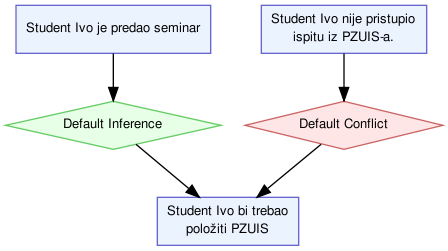
\includegraphics[scale=0.8]{aifdb_ex.png}
\caption{Primjer jednostavnog AIF dokumenta u AIFdb korisničkom sučelju}
\label{fig:aifdb_ex}
\end{figure}

AIFdb\footnote{Dostupan na \url{aifdb.org}} \citep{lawrence2012aifdb} 
je softversko rješenje za pretraživanje, pohranu i vizualizaciju AIF dokumenata te
integraciju s drugim Argument Web alatima. 
Sastoji se od tri dijela:
\begin{enumerate*}
    \item korisničkog sučelja za vizualizaciju AIF dokumenata,
    \item baze podataka koja pohranjuje AIF dokumente i
    \item web servisa koji ima programski pristup bazi podataka.
\end{enumerate*}
Baza podataka pohranjuje dokumente u AIF formatu. 
AIF dokumentima u bazi podataka moguće je pristupati kroz korisničko sučenje 
kroz web preglednik, ili programski, koristeći sučelje web servisa.  
Putem web servisa moguće je pretraživati i pregledavati AIF dokumente. 
U AIFdb moguće je uvesti \engl{import} dokumente u formatima alata 
Carnedeas, Rationale i Araucaria te RDF-XML formatu, te izvoziti \engl{export}
u formatima SVG \engl{support vector graphics}, DOT \engl{graph description language}
RDF te formatima alata Rationale i Carnedeas. 

Korisnik može preko web sučelja dodavati AIFdb korpuse \citep{lawrence2014aifdb}, 
koji grupiraju AIF dokumenate. 
Jedan od korpusa dostupan online u AIFdb-u je i Araucaria korpus koji 
u trenutku pisanja sadrži 662 AIF dokumenta. 
Osim pohranjivanja, razmjene i vizualizacije AIF dokumenata, AIFdb je integriran 
s alatima koji evaluiraju arugment u AIF formatu (više u poglavlju~\ref{chap:eval}). 
Jednostavan primjer AIF dokumenta
pohranjen u AIFdb-u je na slici~\ref{fig:aifdb_ex}. Detalje poput sheme 
baze podataka moguće je pronaći u \citep{lawrence2014aifdb} i na web stranicama
centra za tehnologiju argumentacije \engl{Centre for Argument Techology} 
ARG-tech\footnote{Projekti ARG-techa dostupni na \url{http://www.arg-tech.org/index.php/projects/}}.




